% !TeIX spellcheck = cs_CZ
{\tikzset{external/prefix={tikz/FYZII/}}
 \tikzset{external/figure name/.add={ch09_}{}}
%---------------------------------------------------------------------------------------------------
% file fey2ch09.tex
%---------------------------------------------------------------------------------------------------
%=========================== Kapitola: Elektřina v atmosféře =======================================
\chapter{Elektřina v atmosféře}\label{fyz:IIchaIX}
\minitoc
  \section{Gradient elektrického potenciálu v atmosféře}\label{fyz:IIchaIXsecI}
  \section{Elektrické proudy v atmosféře}\label{fyz:IIchaIXsecII}
  \section{Původ atmosférických proudu}\label{fyz:IIchaIXsecIII}
  \section{Bouřky}\label{fyz:IIchaIXsecIV}
  \section{Mechanismus oddělování nábojů}\label{fyz:IIchaIXsecV}
  \section{Blesk}\label{fyz:IIchaIXsecVI}

    \begin{figure}[ht!]
      \centering
      \begin{tabular}{c}
        \subfloat[ ]{\label{fyz_fig689a}
          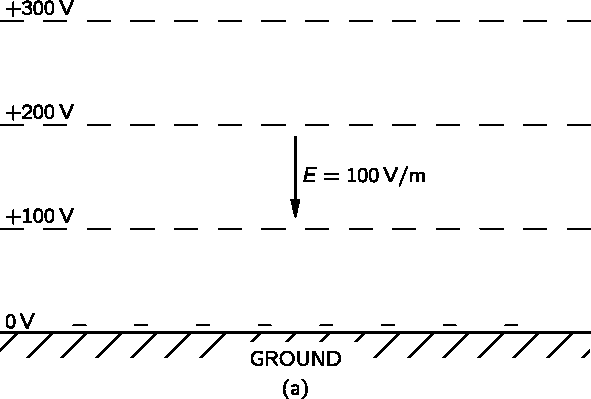
\includegraphics[width=0.6\linewidth]{fyz_fig689a.pdf}}               \\
        \subfloat[ ]{\label{fyz_fig689b}
          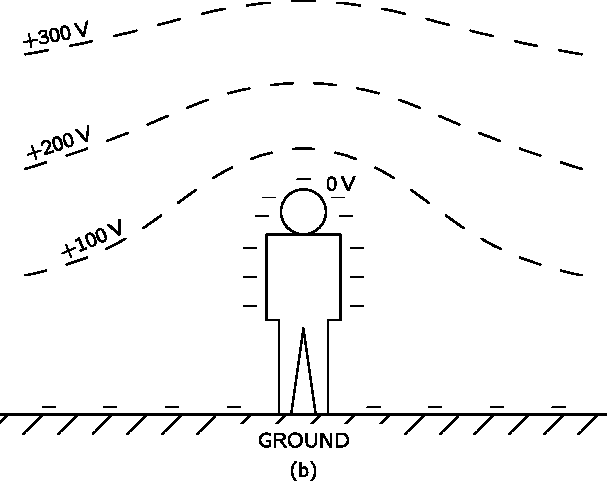
\includegraphics[width=0.6\linewidth]{fyz_fig689b.pdf}}
      \end{tabular}
      \label{fyz_fig689}
      \caption{
               (\cite[s.~748]{Feynman02})}
    \end{figure}

    \begin{figure}[ht!] %\ref{fyz_fig690}
      \centering
      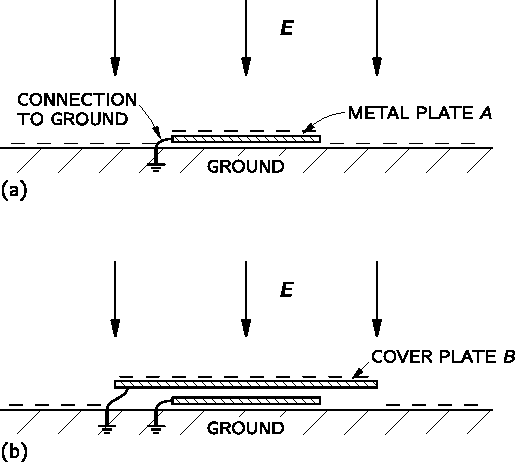
\includegraphics[width=0.7\linewidth]{fyz_fig690.pdf}
      \caption{
               (\cite[s.~707]{Feynman02})}
      \label{fyz_fig690}
    \end{figure}

    \begin{figure}[ht!] %\ref{fyz_fig691}
      \centering
      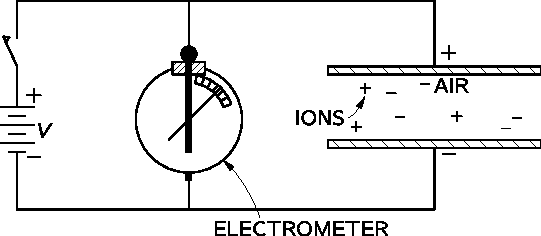
\includegraphics[width=0.7\linewidth]{fyz_fig691.pdf}
      \caption{
               (\cite[s.~707]{Feynman02})}
      \label{fyz_fig691}
    \end{figure}


    \begin{figure}[ht!] %\ref{fyz_fig692}
      \centering
      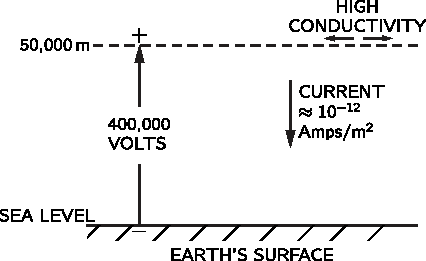
\includegraphics[width=0.7\linewidth]{fyz_fig692.pdf}
      \caption{
               (\cite[s.~707]{Feynman02})}
      \label{fyz_fig692}
    \end{figure}

    \begin{figure}[ht!] %\ref{fyz_fig693}
      \centering
      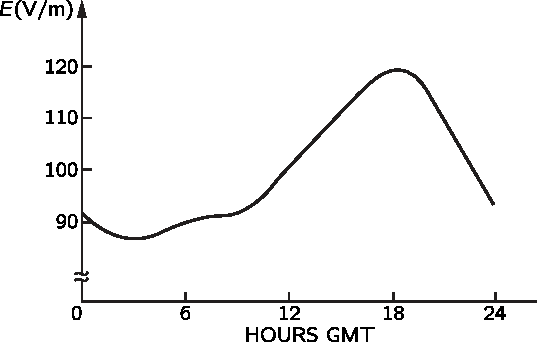
\includegraphics[width=0.7\linewidth]{fyz_fig693.pdf}
      \caption{
               (\cite[s.~707]{Feynman02})}
      \label{fyz_fig693}
    \end{figure}

    \begin{figure}[ht!] %\ref{fyz_fig694}
      \centering
      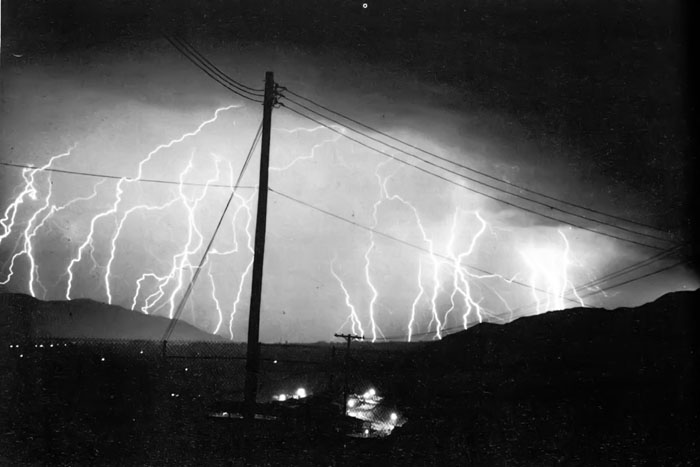
\includegraphics[width=0.7\linewidth]{fyz_fig694.jpg}
      \caption{
               (\cite[s.~707]{Feynman02})}
      \label{fyz_fig694}
    \end{figure}

    \begin{figure}[ht!] %\ref{fyz_fig695}
      \centering
      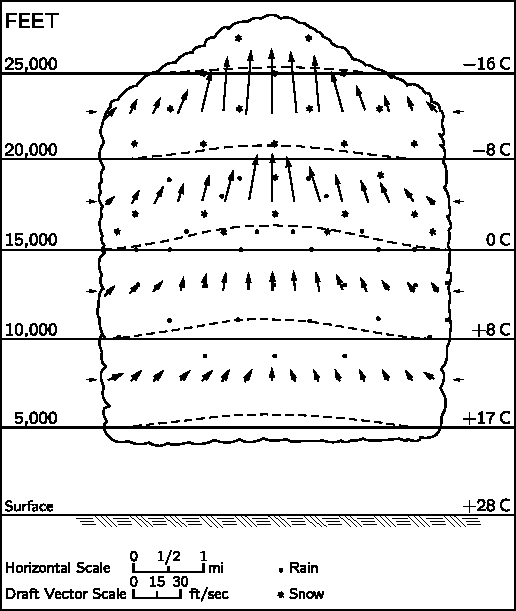
\includegraphics[width=0.7\linewidth]{fyz_fig695.pdf}
      \caption{
               (\cite[s.~707]{Feynman02})}
      \label{fyz_fig695}
    \end{figure}

    \begin{figure}[ht!] %\ref{fyz_fig696}
      \centering
      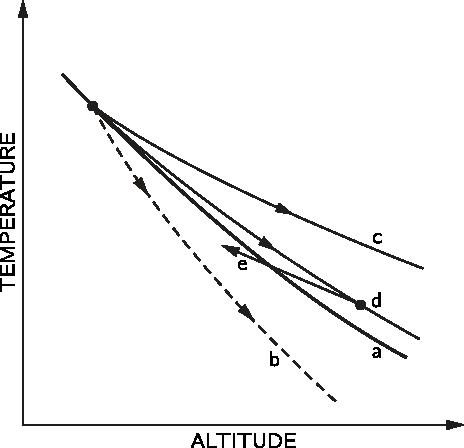
\includegraphics[width=0.7\linewidth]{fyz_fig696.pdf}
      \caption{
               (\cite[s.~707]{Feynman02})}
      \label{fyz_fig696}
    \end{figure}

    \begin{figure}[ht!] %\ref{fyz_fig697}
      \centering
      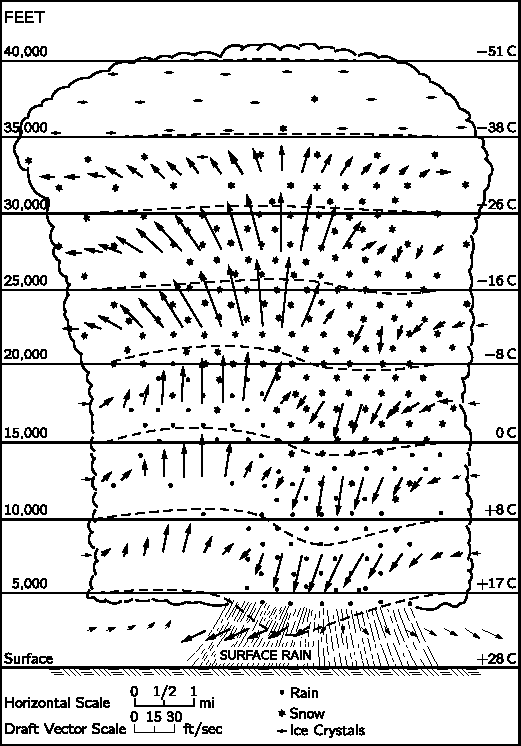
\includegraphics[width=0.7\linewidth]{fyz_fig697.pdf}
      \caption{
               (\cite[s.~707]{Feynman02})}
      \label{fyz_fig697}
    \end{figure}

    \begin{figure}[ht!] %\ref{fyz_fig698}
      \centering
      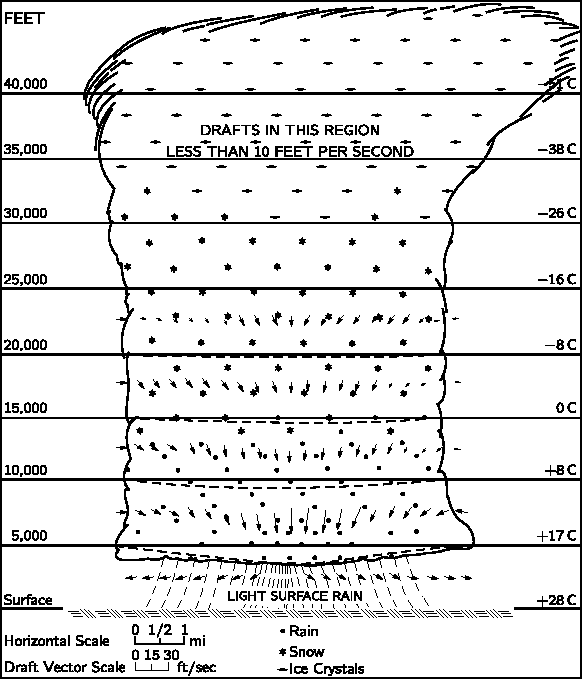
\includegraphics[width=0.7\linewidth]{fyz_fig698.pdf}
      \caption{
               (\cite[s.~707]{Feynman02})}
      \label{fyz_fig698}
    \end{figure}

    \begin{figure}[ht!] %\ref{fyz_fig699}
      \centering
      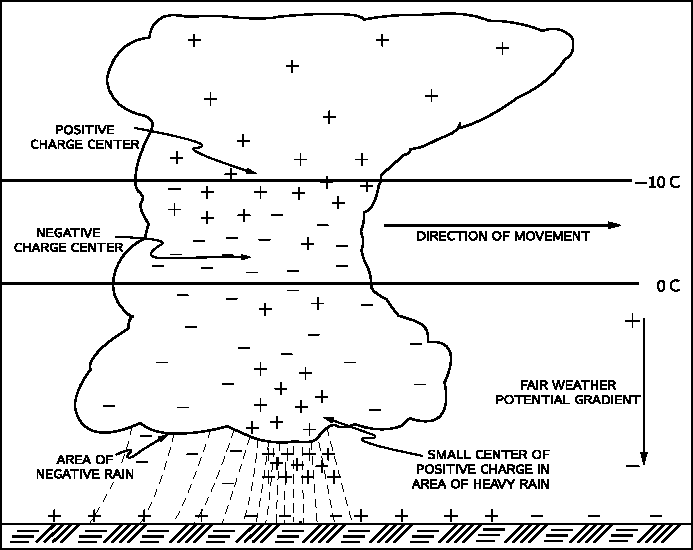
\includegraphics[width=0.7\linewidth]{fyz_fig699.pdf}
      \caption{
               (\cite[s.~707]{Feynman02})}
      \label{fyz_fig699}
    \end{figure}

    \begin{figure}[ht!] %\ref{fyz_fig700}
      \centering
      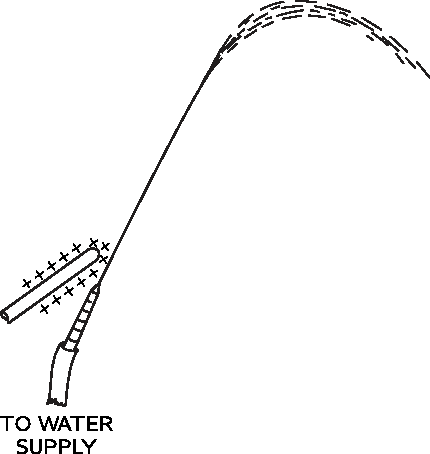
\includegraphics[width=0.7\linewidth]{fyz_fig700.pdf}
      \caption{
               (\cite[s.~707]{Feynman02})}
      \label{fyz_fig700}
    \end{figure}

    \begin{figure}[ht!] %\ref{fyz_fig701}
      \centering
      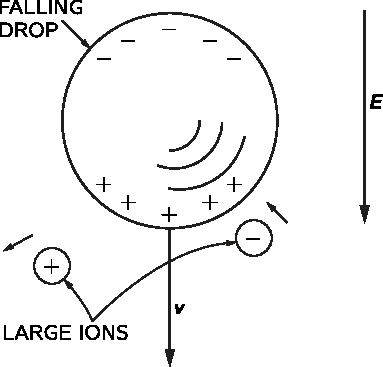
\includegraphics[width=0.7\linewidth]{fyz_fig701.pdf}
      \caption{
               (\cite[s.~707]{Feynman02})}
      \label{fyz_fig701}
    \end{figure}

    \begin{figure}[ht!] %\ref{fyz_fig702}
      \centering
      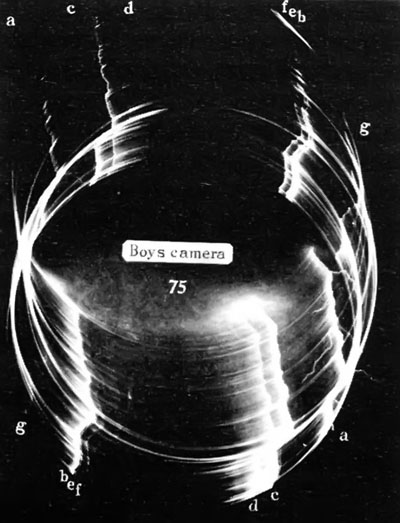
\includegraphics[width=0.7\linewidth]{fyz_fig702.jpg}
      \caption{
               (\cite[s.~707]{Feynman02})}
      \label{fyz_fig702}
    \end{figure}

    \begin{figure}[ht!] %\ref{fyz_fig703}
      \centering
      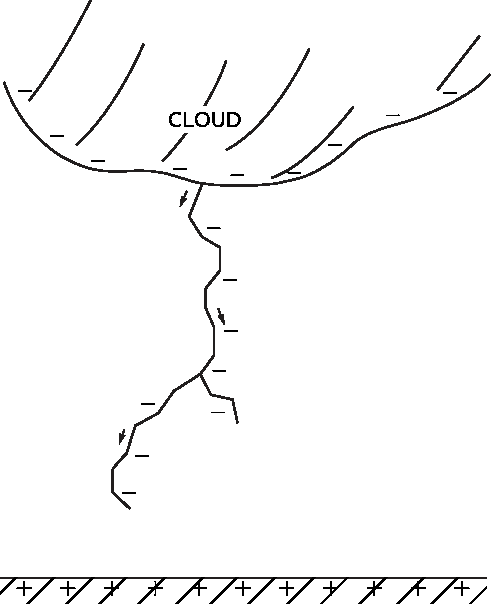
\includegraphics[width=0.7\linewidth]{fyz_fig703.pdf}
      \caption{
               (\cite[s.~707]{Feynman02})}
      \label{fyz_fig703}
    \end{figure}

    \begin{figure}[ht!] %\ref{fyz_fig704}
      \centering
      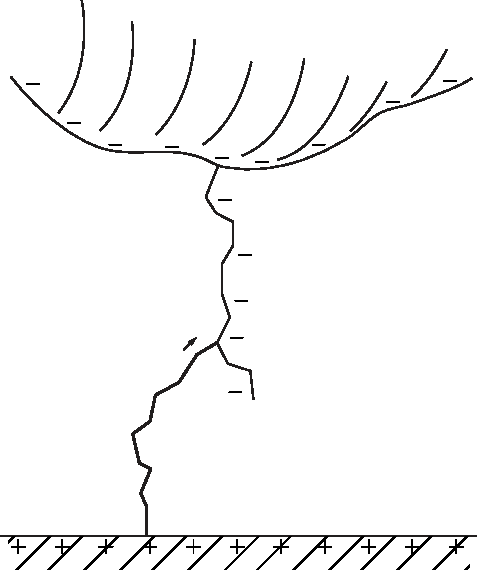
\includegraphics[width=0.7\linewidth]{fyz_fig704.pdf}
      \caption{
               (\cite[s.~707]{Feynman02})}
      \label{fyz_fig704}
    \end{figure}


} %tikzset
%---------------------------------------------------------------------------------------------------
%\printbibliography[title={Seznam literatury},heading=subbibliography]
\addcontentsline{toc}{section}{Seznam literatury}